%%%
% Plantilla de Trabajo
% Modificación de una plantilla de Latex de Frits Wenneker para adaptarla 
% al castellano y a las necesidades de escribir informática y matemáticas.
%
% Editada por: Mario Román
%
% License:
% CC BY-NC-SA 3.0 (http://creativecommons.org/licenses/by-nc-sa/3.0/)
%%%

%%%%%%%%%%%%%%%%%%%%%%%%%%%%%%%%%%%%%%%%
% Short Sectioned Assignment
% LaTeX Template
% Version 1.0 (5/5/12)
%
% This template has been downloaded from:
% http://www.LaTeXTemplates.com
%
% Original author:
% Frits Wenneker (http://www.howtotex.com)
%
% License:
% CC BY-NC-SA 3.0 (http://creativecommons.org/licenses/by-nc-sa/3.0/)
%
%%%%%%%%%%%%%%%%%%%%%%%%%%%%%%%%%%%%%%%%%

%----------------------------------------------------------------------------------------
%	PAQUETES Y CONFIGURACIÓN DEL DOCUMENTO
%----------------------------------------------------------------------------------------

%%% Configuración del papel.
% fourier: Usa la fuente Adobe Utopia. (Comentando la línea usa la fuente normal)
\documentclass[paper=a4, fontsize=11pt, spanish]{scrartcl} 
\usepackage{fourier}

% Centra y formatea los títulos de sección.
% Quita la indentación de párrafos.
\usepackage{sectsty} % Allows customizing section commands
\allsectionsfont{\centering \normalfont\scshape} % Make all sections centered, the default font and small caps
\setlength\parindent{0pt} % Removes all indentation from paragraphs - comment this line for an assignment with lots of text

% Permite elegir cabeceras y pies de página.
\usepackage{fancyhdr} % Custom headers and footers
\pagestyle{fancyplain} % Makes all pages in the document conform to the custom headers and footers
\fancyhead{} % No page header - if you want one, create it in the same way as the footers below
\fancyfoot[L]{} % Empty left footer
\fancyfoot[C]{} % Empty center footer
\fancyfoot[R]{\thepage} % Page numbering for right footer
\renewcommand{\headrulewidth}{0pt} % Remove header underlines
\renewcommand{\footrulewidth}{0pt} % Remove footer underlines
\setlength{\headheight}{13.6pt} % Customize the height of the header


%%% Castellano.
% noquoting: Permite uso de comillas no españolas.
% lcroman: Permite la enumeración con numerales romanos en minúscula.
% fontenc: Usa la fuente completa para que pueda copiarse correctamente del pdf.
\usepackage[spanish,es-noquoting,es-lcroman]{babel}
\usepackage[utf8]{inputenc}
\usepackage[T1]{fontenc}
\selectlanguage{spanish}


%%% Matemáticas.
% Paquetes de la AMS. Para entornos de ecuaciones.
\usepackage{amsmath,amsfonts,amsthm}

% Incluye números entre secciones y ecuaciones.
\numberwithin{equation}{section} % Number equations within sections (i.e. 1.1, 1.2, 2.1, 2.2 instead of 1, 2, 3, 4)
\numberwithin{figure}{section} % Number figures within sections (i.e. 1.1, 1.2, 2.1, 2.2 instead of 1, 2, 3, 4)
\numberwithin{table}{section} % Number tables within sections (i.e. 1.1, 1.2, 2.1, 2.2 instead of 1, 2, 3, 4)

%%% Códigos C / C++ / SQL ...
% Paquete listings para visualización de código más elegante
\usepackage{xcolor,listings}
\usepackage{textcomp}
\lstset{upquote=true}

%% Gráficos e imagenes:
\usepackage{graphicx}


%----------------------------------------------------------------------------------------
%	TÍTULO
%----------------------------------------------------------------------------------------
% Título con las líneas horizontales, nombres y fecha.

\newcommand{\horrule}[1]{\rule{\linewidth}{#1}} % Create horizontal rule command with 1 argument of height

\title{
  \normalfont \normalsize 
  \textsc{Universidad de Granada.\\Sistemas Multidimensionales} \\ [25pt] % Your university, school and/or department name(s)
  \horrule{0.5pt} \\[0.4cm] % Thin top horizontal rule
  \huge Práctica 3: Diseño e implementación de esquemas de bases de datos multidimensionales. \\ % The assignment title
  \horrule{2pt} \\[0.5cm] % Thick bottom horizontal rule
}

\author{Daniel López García\\Rafael Nogales Vaquero} % Your name

\date{\normalsize\today} % Today's date or a custom date



%----------------------------------------------------------------------------------------
%	DOCUMENTO
%----------------------------------------------------------------------------------------


\begin{document}
\maketitle % Escribe el título
\newpage
\textbf{1. Implementar, de manera coherente con el diseño conceptual citado y la base de datos aportada, un cubo multidimensional mediante la herramienta Excel.}\\

En primer lugar usamos Access para obtener las tablas del modelo conceptual. Para obtener la dimensión Cuando haremos una consulta en la tabla LineaDeVenta. La vista del Diseño de la consulta es la siguiente:

\begin{center}
	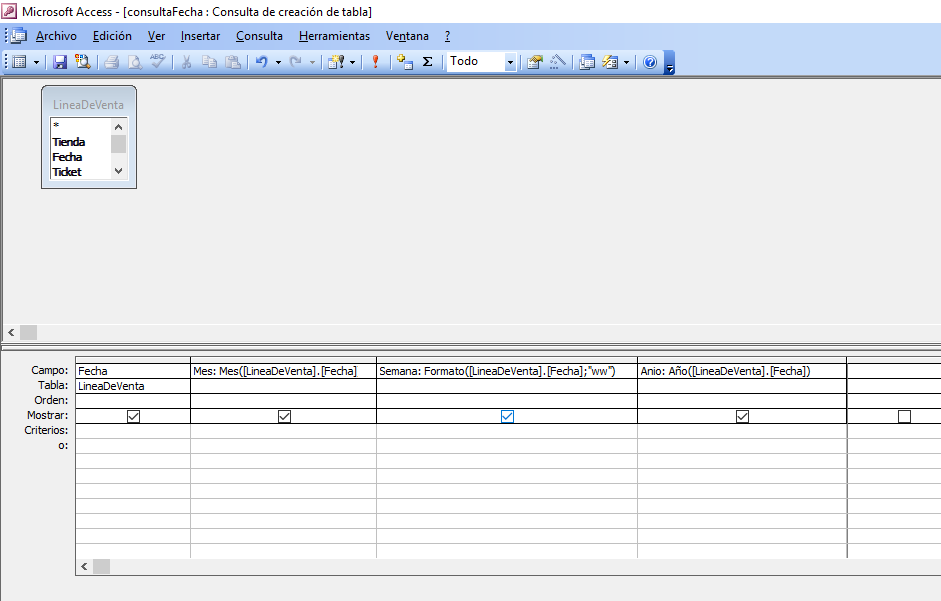
\includegraphics[scale=0.5]{img1.png}
\end{center}
El código SQL generado para la consulta es el siguiente:
\begin{lstlisting}[
language=SQL,
breaklines=true,
showspaces=false,
basicstyle=\ttfamily,
numbers=left,
numberstyle=\tiny,
commentstyle=\color{gray}
]
SELECT DISTINCT LineaDeVenta.Fecha, Month([LineaDeVenta].[Fecha]) AS Mes, Format([LineaDeVenta].[Fecha],"ww") AS Semana, Year([LineaDeVenta].[Fecha]) AS Anio INTO Fecha
FROM LineaDeVenta;
\end{lstlisting}

Podemos ver el resultado de la ejecución de la consulta en las siguiente imagen:\\
\\
\begin{center}
	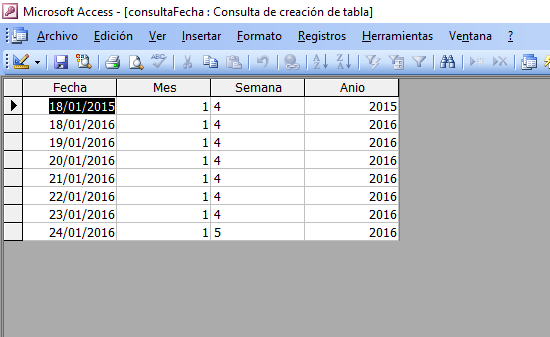
\includegraphics[scale=0.75]{img2.png}
\end{center}
\bigskip

A continuación, hacemos otra consulta para la creación de la tabla Venta usando las claves autogeneradas de las tablas Libro, Fecha y Tienda y añadiendo las mediciones(teniendo en cuenta su aditividad).
\begin{center}
	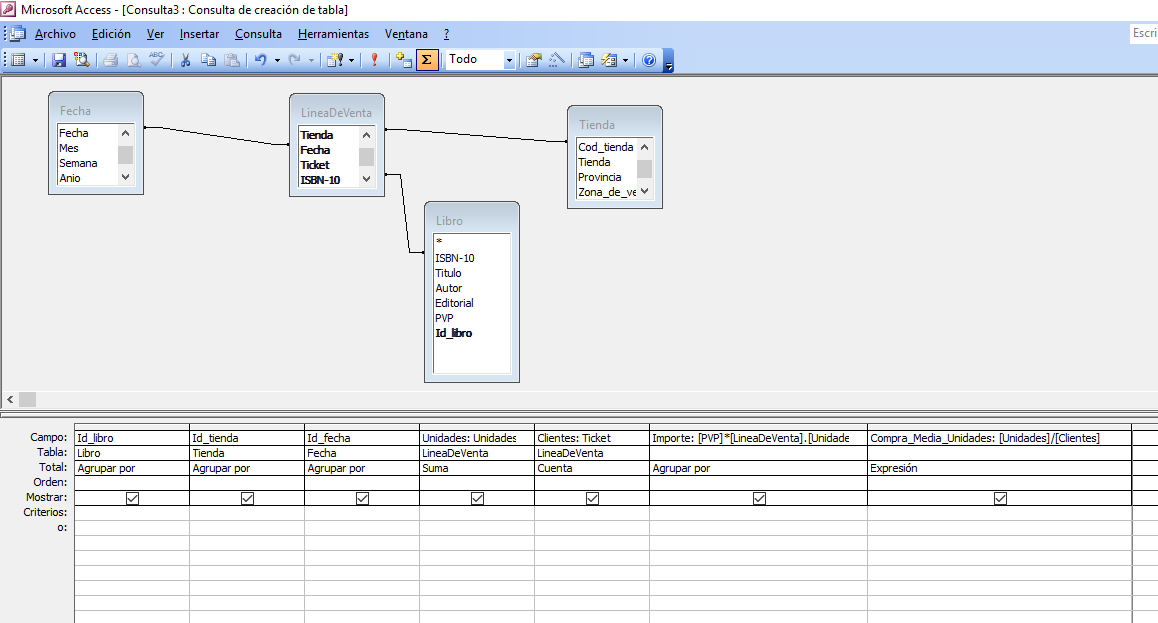
\includegraphics[scale=0.5]{img3.png}
\end{center}
El código SQL generado para la consulta es el siguiente:
\begin{lstlisting}[
language=SQL,
breaklines=true,
showspaces=false,
basicstyle=\ttfamily,
numbers=left,
numberstyle=\tiny,
commentstyle=\color{gray}
]
SELECT Libro.Id_libro, Tienda.Id_tienda, Fecha.Id_fecha, Sum(LineaDeVenta.Unidades) AS Unidades, Count(LineaDeVenta.Ticket) AS Clientes, [PVP]*[LineaDeVenta].[Unidades] AS Importe, [Unidades]/[Clientes] AS Compra_Media_Unidades INTO Venta
FROM Fecha INNER JOIN (Tienda INNER JOIN (Libro INNER JOIN LineaDeVenta ON Libro.[ISBN-10] = LineaDeVenta.[ISBN-10]) ON Tienda.Cod_tienda = LineaDeVenta.Tienda) ON Fecha.Fecha = LineaDeVenta.Fecha
GROUP BY Libro.Id_libro, Tienda.Id_tienda, Fecha.Id_fecha, [PVP]*[LineaDeVenta].[Unidades];
\end{lstlisting}
Podemos ver el resultado de la ejecución de la consulta en las siguiente imagen:\\
\\
\begin{center}
	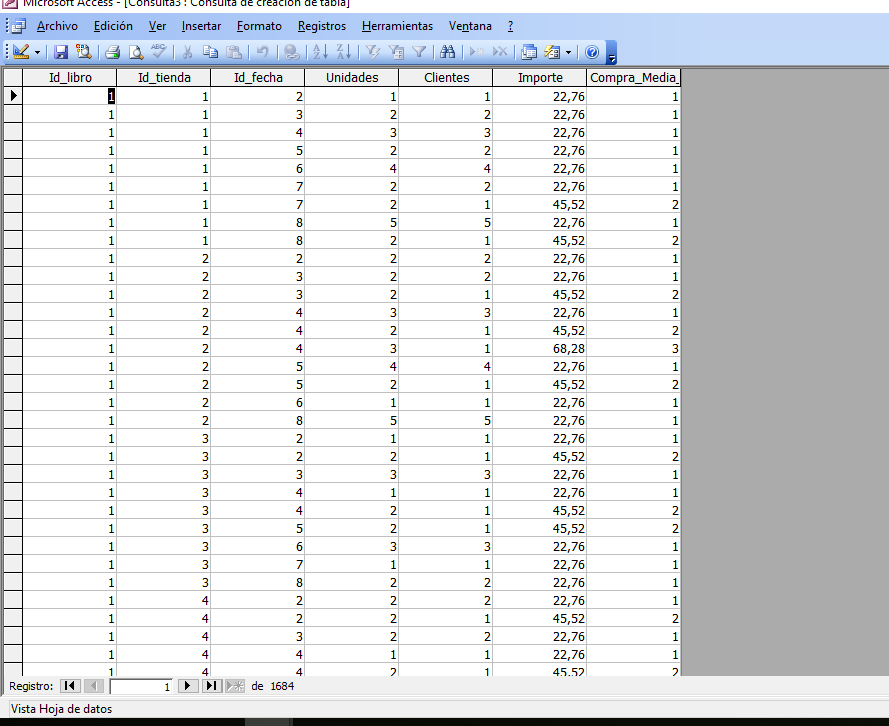
\includegraphics[scale=0.5]{img4.png}
\end{center}
\bigskip 

Finalmente, creamos la consulta que usará Excel. Para ello debemos tener en cuenta que cada jerarquía debe ser considerada cómo una dimensión y que la fecha debe estar en formato texto. 
El código SQL generado para la consulta es el siguiente:

\begin{lstlisting}[
language=SQL,
breaklines=true,
showspaces=false,
basicstyle=\ttfamily,
numbers=left,
numberstyle=\tiny,
commentstyle=\color{gray}
]
SELECT Libro.Titulo, Libro.Autor, Tienda.Tienda AS Tienda1, Tienda.Zona_de_ventas, Tienda.Tienda, Tienda.Provincia, Fecha.Fecha AS Fecha1, Fecha.Mes, Fecha.Anio AS Anio1, Format([Fecha].[Fecha],"dd/mm/yyyy") AS Fecha, Fecha.Semana, Fecha.Anio, Venta.Unidades, Venta.Clientes, Venta.Importe, Venta.Compra_Media_Unidades
FROM Fecha INNER JOIN ((Venta INNER JOIN Tienda ON Venta.Id_tienda = Tienda.Id_tienda) INNER JOIN Libro ON Venta.Id_libro = Libro.Id_libro) ON Fecha.Id_fecha = Venta.Id_fecha;
\end{lstlisting}
La vista de diseño de la consulta y el resultado de la misma se puede observar en las siguientes imágenes:\\
\begin{center}
	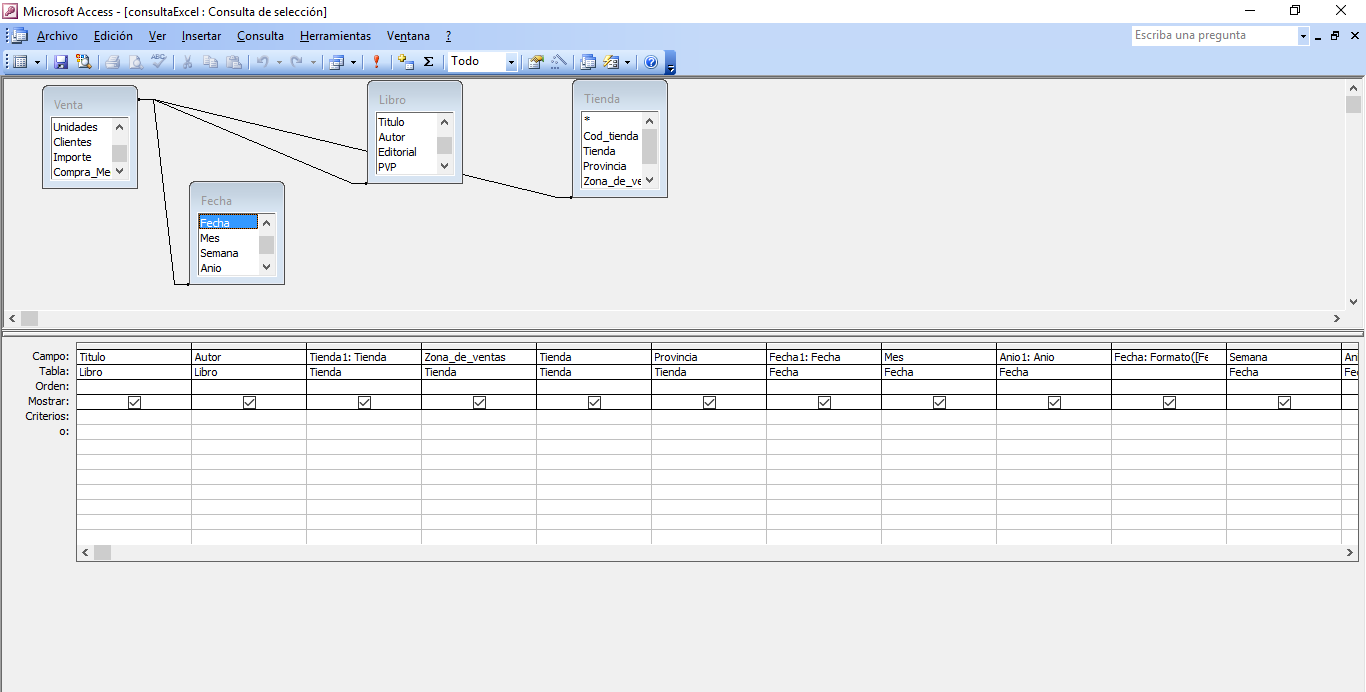
\includegraphics[scale=0.5]{img5.png}
	
	\medskip
	
	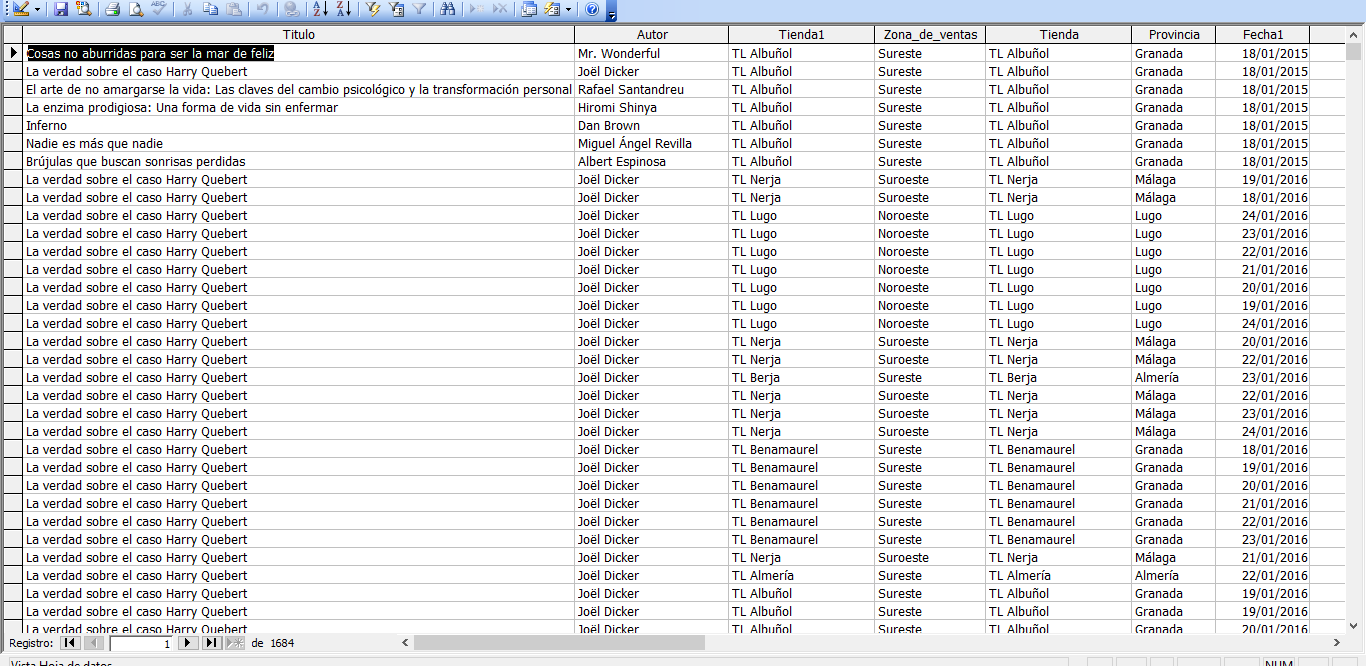
\includegraphics[scale=0.5]{img6.png}
\end{center}
Ahora desde la herramienta Excel, creamos el cubo OLAP añadiendo las dimensiones y las mediciones, cómo se muestra en las siguientes imágenes. Dado que para añadir la medición Compra\_Media\_Unidades(no aditiva, por ser una media), debemos seleccionar una función para resumir los datos hemos seleccionado la función máximo.
\begin{center}
	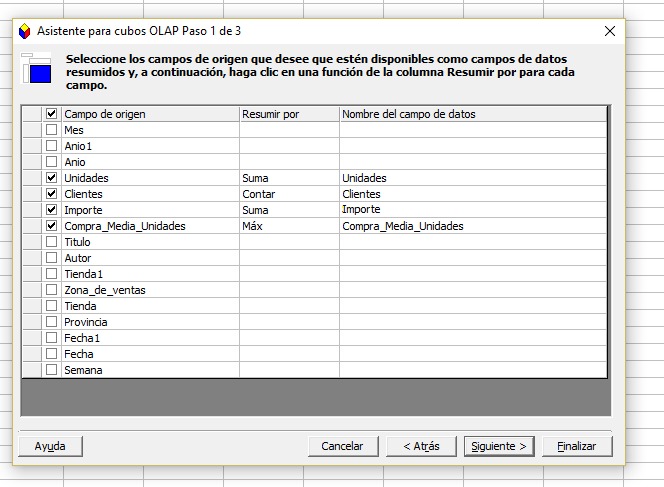
\includegraphics[scale=0.75]{img7.png}
	
	\medskip 	
	
	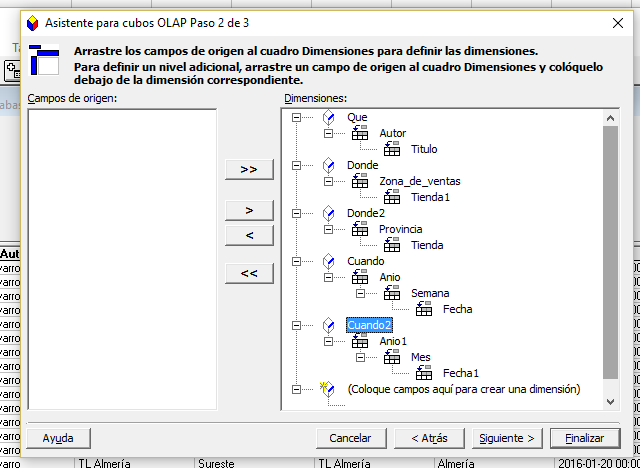
\includegraphics[scale=0.75]{img8.png}
\end{center}

\textbf{2. Partiendo de un informe en blanco y haciendo uso de la implementación anterior y de una tabla dinámica asociada al cubo, se desea tener el siguiente informe: “Importe de las ventas y compra media de unidades por tienda el 18 de enero de 2015 y el 18 de enero de 2016”.}
\\
El nivel del cubo inicial es Qué:Todo, Cuando:Todo, Dónde:Todo. En primer lugar añadimos las mediciones al área de datos. A continuación, agregamos la dimensión Dónde(en nuestro caso Donde2) al área de filas. Hemos efectuado una operación drill-down y el nivel de cubo es Qué:Todo,Cuando:Todo,Dónde:Provincia. Para mostrar las tiendas seleccionamos Mostrar detalle. De nuevo es una operación drill-down y el nivel de cubo es Qué:Todo, Cuando:Todo, Dónde:Tienda. Para ver sólo las tiendas en el informe seleccionamos la opción Ocultar niveles sobre Provincia. No es una operación y por tanto el nivel del cubo no cambia.\\
Finalmente, añadimos la dimensión Cuando al área de páginas y seleccionamos las fechas deseadas. Es una operación slice\&dice y el nivel del cubo no varía.\\
\\
El resultado del informe es el siguiente:
\\
\begin{center}
	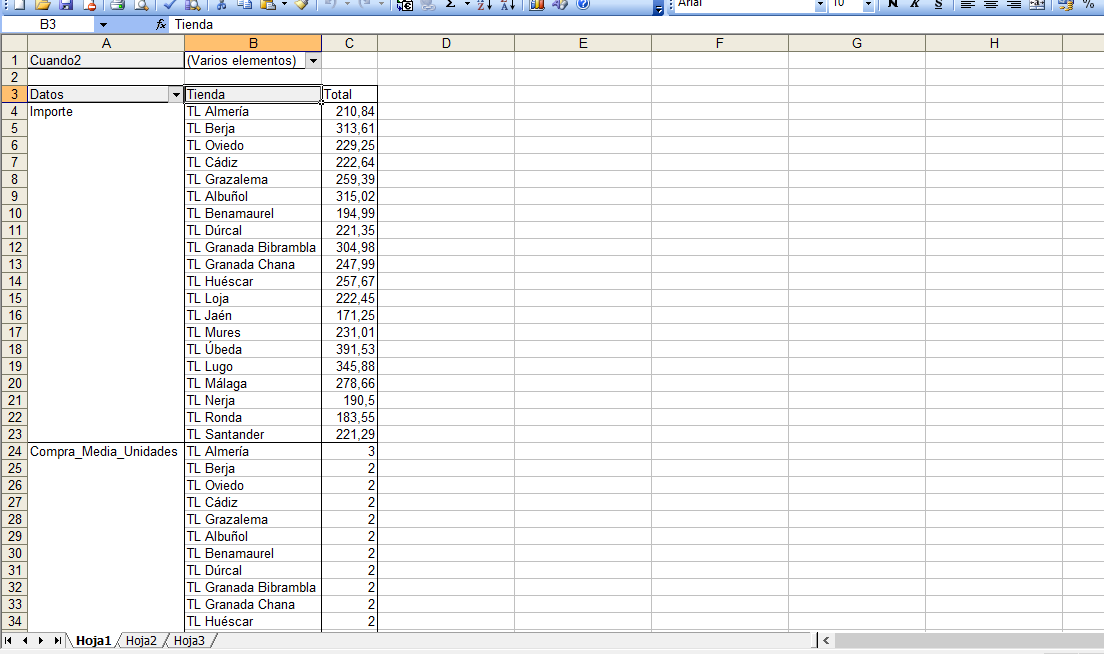
\includegraphics[scale=0.75]{img9.png}
\end{center}


\textbf{3. A partir del informe anterior, se pide la definición y generación de una secuencia de informes donde se documente el uso de las operaciones Drill Down, Roll Up y Slice \& Dice, indicando, paso a paso, la operación que se aplica y el cubo obtenido en cada caso, e incluyendo las copias de pantalla donde se pueda ver la evolución de la secuencia de informes y el informe final generado.}
\\
El nivel original del cubo es el mismo que teníamos al final del ejercicio 2: Qué:Todo, Cuando:Todo, Dónde:Tienda.\\
En primer lugar vamos a realizar una operación drill-down en la que mostraremos el detalle de las provincias (moviendonos en dos jerarquías)
Ahora el nivel del cubo es: Qué:Todo, Cuando:Todo, Dónde:Tienda y Provincia.

\begin{center}
	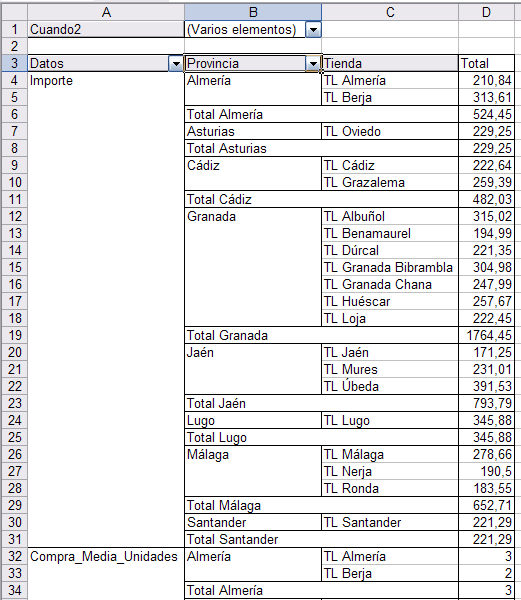
\includegraphics[scale=0.75]{drillDown.png}
\end{center}

Ahora vamos a hacer slice \& dice y vamos a seleccionar únicamente las tiendas de la provincia de Granada.\\
Como sabemos el nivel del cubo no cambia.
\begin{center}
	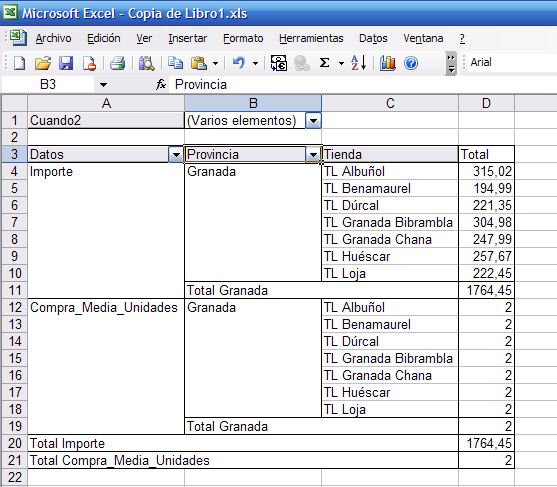
\includegraphics[scale=0.75]{slice&dice.png}
\end{center}
	
Por último vamos a hacer roll-up por la dimension Donde y vamos a eliminar el detalle de las tiendas.
La dimension del cubo es: Qué:Todo, Cuando:Todo, Dónde:Provincia.

\begin{center}
	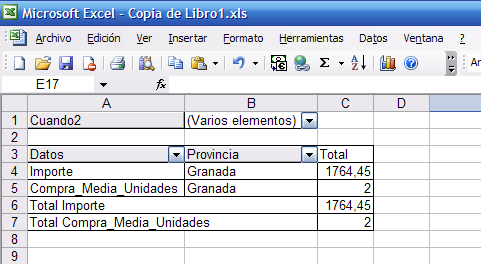
\includegraphics[scale=0.75]{rollup.png}
\end{center}
	

\end{document}
